\documentclass[border=4pt]{standalone}
\usepackage[T1]{fontenc}
\usepackage{lmodern}
\usepackage{amsmath}
\usepackage{pgfplots}
\pgfplotsset{compat=1.18}
\usepgfplotslibrary{groupplots,fillbetween}
\usetikzlibrary{calc,arrows.meta}
% one colour per kind of method, the same in every figure (Okabe-Ito)
\definecolor{neur}{HTML}{D55E00}   % neurons chosen by attribution
\definecolor{dirc}{HTML}{009E73}   % directions from the weird-vs-normal contrast
\definecolor{read}{HTML}{0072B2}   % readout methods and interventions chosen from readouts
\definecolor{pers}{HTML}{CC79A7}   % Assistant Axis / persona
\definecolor{ctrl}{HTML}{8C8C8C}   % random controls
\definecolor{meas}{HTML}{E69F00}   % measured outcome
\definecolor{ink}{HTML}{222222}
\pgfplotsset{
  every axis/.append style={clip=false, font=\small, axis line style={black!55}, tick style={black!55}, tick align=outside,
    label style={font=\small}, tick label style={font=\footnotesize}, title style={font=\small, align=center}},
  grid style={black!9, line width=0.4pt},
  every axis legend/.append style={font=\footnotesize, draw=none, fill=none},
  ci/.style={/pgfplots/error bars/x dir=both, /pgfplots/error bars/x explicit, /pgfplots/error bars/error bar style={line width=0.8pt}, /pgfplots/error bars/error mark=none},
  yci/.style={/pgfplots/error bars/y dir=both, /pgfplots/error bars/y explicit, /pgfplots/error bars/error bar style={line width=0.8pt}, /pgfplots/error bars/error mark=none},
}

\begin{document}
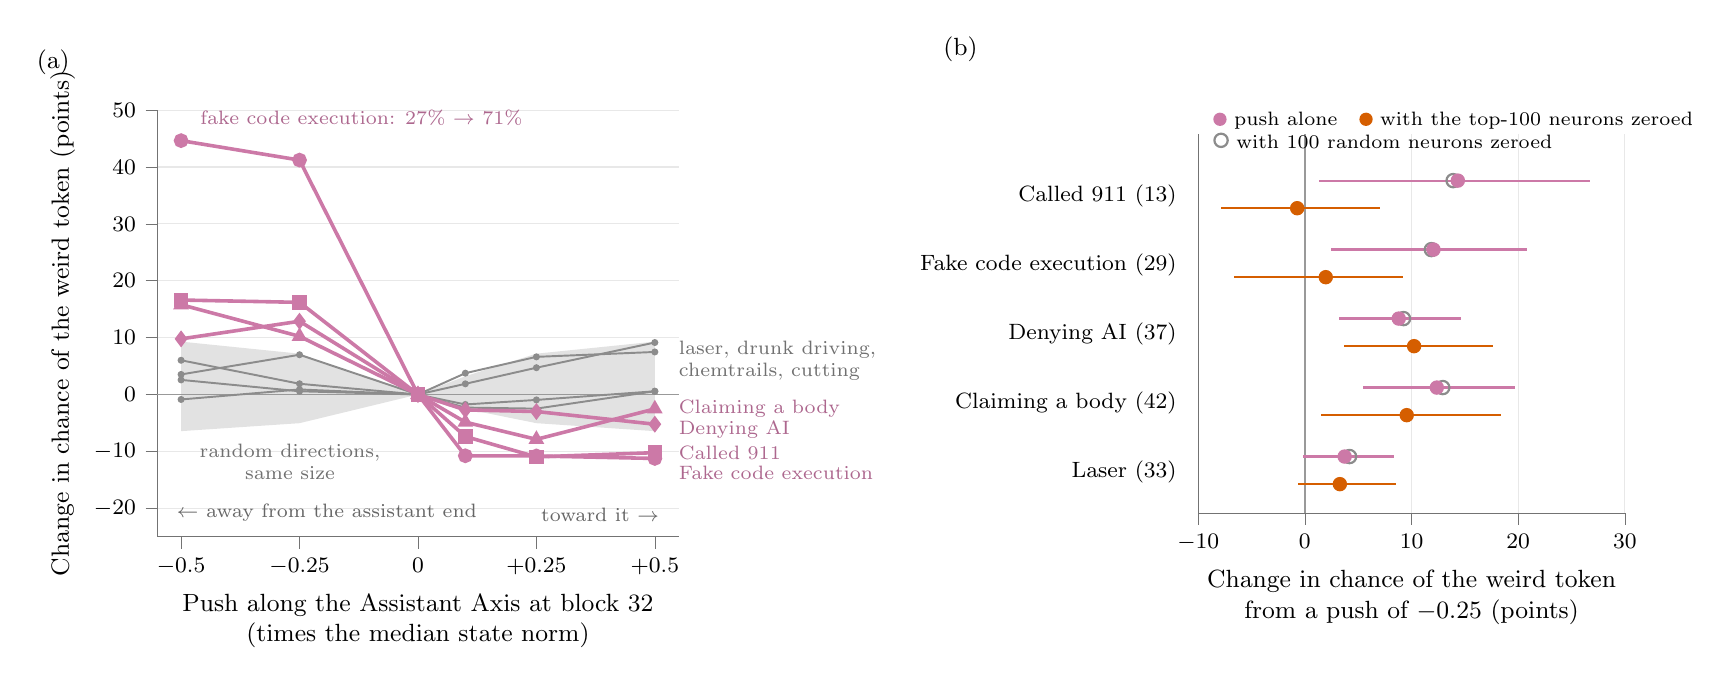
\begin{tikzpicture}
\begin{axis}[name=a, width=8.2cm, height=7cm, xmin=-0.55, xmax=0.55, xtick={-0.5,-0.25,0,0.25,0.5}, xticklabels={$-0.5$,$-0.25$,0,$+0.25$,$+0.5$}, ymin=-25, ymax=50, ytick={-20,-10,0,10,20,30,40,50}, yticklabel={$\pgfmathprintnumber{\tick}$}, axis x line*=bottom, axis y line*=left, ymajorgrids, xlabel={Push along the Assistant Axis at block 32\\(times the median state norm)}, xlabel style={align=center}, ylabel={Change in chance of the weird token (points)}, title={(a)}, title style={at={(-0.25,1.02)}, anchor=south west}]
\addplot[name path=bu, draw=none] coordinates {(-0.5,9.30) (-0.25,7.18) (0.0,0.00) (0.1,3.21) (0.25,7.18) (0.5,9.30)};
\addplot[name path=bd, draw=none] coordinates {(-0.5,-6.44) (-0.25,-5.04) (0.0,0.00) (0.1,-2.52) (0.25,-5.04) (0.5,-6.44)};
\addplot[ctrl, fill opacity=0.25] fill between[of=bu and bd];
\draw[black!40, line width=0.5pt] (axis cs:-0.55,0) -- (axis cs:0.55,0);
\node[font=\scriptsize, black!60, anchor=south west] at (axis cs:-0.53,-24) {$\leftarrow$ away from the assistant end};
\node[font=\scriptsize, black!60, anchor=south east] at (axis cs:0.53,-24) {toward it $\rightarrow$};
\node[font=\scriptsize, ctrl!80!black, anchor=north, align=center] at (axis cs:-0.27,-7) {random directions,\\same size};
\node[font=\scriptsize, pers!85!black, anchor=south west, align=left] at (axis cs:-0.48,45.63) {fake code execution: 27\% $\to$ 71\%};
\addplot[ctrl, line width=0.7pt, mark=*, mark size=0.9pt] coordinates {(-0.5,3.53) (-0.25,6.99) (0.0,0.00) (0.1,-2.30) (0.25,-2.48) (0.5,0.58)};
\addplot[ctrl, line width=0.7pt, mark=*, mark size=0.9pt] coordinates {(-0.5,2.57) (-0.25,0.57) (0.0,0.00) (0.1,1.88) (0.25,4.71) (0.5,9.14)};
\addplot[ctrl, line width=0.7pt, mark=*, mark size=0.9pt] coordinates {(-0.5,-0.87) (-0.25,0.89) (0.0,0.00) (0.1,-1.75) (0.25,-0.95) (0.5,0.57)};
\addplot[ctrl, line width=0.7pt, mark=*, mark size=0.9pt] coordinates {(-0.5,6.02) (-0.25,1.89) (0.0,0.00) (0.1,3.75) (0.25,6.62) (0.5,7.48)};
\addplot[pers, line width=1.3pt, mark=*, mark size=2pt] coordinates {(-0.5,44.63) (-0.25,41.21) (0.0,0.00) (0.1,-10.77) (0.25,-10.80) (0.5,-11.24)};
\addplot[pers, line width=1.3pt, mark=square*, mark size=2pt] coordinates {(-0.5,16.61) (-0.25,16.20) (0.0,0.00) (0.1,-7.38) (0.25,-10.97) (0.5,-10.22)};
\addplot[pers, line width=1.3pt, mark=triangle*, mark size=2pt] coordinates {(-0.5,15.79) (-0.25,10.23) (0.0,0.00) (0.1,-4.86) (0.25,-7.88) (0.5,-2.53)};
\addplot[pers, line width=1.3pt, mark=diamond*, mark size=2pt] coordinates {(-0.5,9.78) (-0.25,12.88) (0.0,0.00) (0.1,-2.71) (0.25,-2.99) (0.5,-5.22)};
\node[font=\scriptsize, pers!85!black, anchor=west] at (axis cs:0.53,-2.53) {Claiming a body};
\node[font=\scriptsize, pers!85!black, anchor=west] at (axis cs:0.53,-6.13) {Denying AI};
\node[font=\scriptsize, pers!85!black, anchor=west] at (axis cs:0.53,-10.22) {Called 911};
\node[font=\scriptsize, pers!85!black, anchor=west] at (axis cs:0.53,-13.82) {Fake code execution};
\node[font=\scriptsize, ctrl!80!black, anchor=west, align=left] at (axis cs:0.53,6) {laser, drunk driving,\\chemtrails, cutting};
\end{axis}
\begin{axis}[at={($(a.east)+(6.6cm,0)$)}, anchor=west, width=7cm, height=6.4cm, xmin=-10, xmax=30, xtick={-10,0,10,20,30}, ymin=-4.6, ymax=0.9, ytick={0,-1,-2,-3,-4}, yticklabels={{Called 911 (13)},{Fake code execution (29)},{Denying AI (37)},{Claiming a body (42)},{Laser (33)}}, y tick label style={font=\footnotesize}, major y tick style={draw=none}, axis x line*=bottom, axis y line*=left, xmajorgrids, xlabel={Change in chance of the weird token\\from a push of $-0.25$ (points)}, xlabel style={align=center}, title={(b)}, title style={at={(-0.62,1.12)}, anchor=south west}]
\draw[black!40, line width=0.5pt] (axis cs:0,-4.6) -- (axis cs:0,0.9);
\addplot[only marks, mark=o, mark size=2.4pt, ctrl, line width=0.8pt] coordinates {(13.90,0.22)};
\addplot[only marks, mark=*, mark size=2.4pt, pers, ci] coordinates {(14.34,0.22) += (12.39,0) -= (13.00,0)};
\addplot[only marks, mark=*, mark size=2.4pt, neur, ci] coordinates {(-0.72,-0.18) += (7.81,0) -= (7.16,0)};
\addplot[only marks, mark=o, mark size=2.4pt, ctrl, line width=0.8pt] coordinates {(11.86,-0.78)};
\addplot[only marks, mark=*, mark size=2.4pt, pers, ci] coordinates {(12.06,-0.78) += (8.79,0) -= (9.60,0)};
\addplot[only marks, mark=*, mark size=2.4pt, neur, ci] coordinates {(1.96,-1.18) += (7.23,0) -= (8.59,0)};
\addplot[only marks, mark=o, mark size=2.4pt, ctrl, line width=0.8pt] coordinates {(9.25,-1.78)};
\addplot[only marks, mark=*, mark size=2.4pt, pers, ci] coordinates {(8.80,-1.78) += (5.82,0) -= (5.61,0)};
\addplot[only marks, mark=*, mark size=2.4pt, neur, ci] coordinates {(10.24,-2.18) += (7.41,0) -= (6.55,0)};
\addplot[only marks, mark=o, mark size=2.4pt, ctrl, line width=0.8pt] coordinates {(12.93,-2.78)};
\addplot[only marks, mark=*, mark size=2.4pt, pers, ci] coordinates {(12.37,-2.78) += (7.33,0) -= (6.91,0)};
\addplot[only marks, mark=*, mark size=2.4pt, neur, ci] coordinates {(9.55,-3.18) += (8.88,0) -= (8.08,0)};
\addplot[only marks, mark=o, mark size=2.4pt, ctrl, line width=0.8pt] coordinates {(4.19,-3.78)};
\addplot[only marks, mark=*, mark size=2.4pt, pers, ci] coordinates {(3.73,-3.78) += (4.67,0) -= (3.90,0)};
\addplot[only marks, mark=*, mark size=2.4pt, neur, ci] coordinates {(3.28,-4.18) += (5.24,0) -= (3.95,0)};
\node[font=\scriptsize, anchor=south west, align=left] at (axis cs:-9.5,0.55) {\tikz\fill[pers] (0,0) circle (2.4pt); push alone\quad \tikz\fill[neur] (0,0) circle (2.4pt); with the top-100 neurons zeroed\\ \tikz\draw[ctrl, line width=0.8pt] (0,0) circle (2.4pt); with 100 random neurons zeroed};
\end{axis}
\end{tikzpicture}
\end{document}
